\documentclass{article}
\usepackage[dblblindworkshop]{neurips_2026}
\workshoptitle{Algorithms for Human-AI Collaboration (AIMS 2026)}

\usepackage[utf8]{inputenc}
\usepackage[T1]{fontenc}
\usepackage{hyperref}
\usepackage{url}
\usepackage{booktabs}
\usepackage{amsfonts}
\usepackage{amsmath}
\usepackage{microtype}
\usepackage{graphicx}
\usepackage{xcolor}
\usepackage{siunitx}

\title{Fair and Transparent Human--AI Collaboration for Personalized Exercise Recommendation via Knowledge Tracing}

\author{
  Joel Gedeon \\
  AIMS 2026 Final Project \\
  \texttt{joel.gedeon@example.com}
}

\begin{document}

\maketitle

\begin{abstract}
This project studies cost-sensitive collaboration for educational recommendation, where the primary objective is to identify whether each student is proficient on a target skill (needs support or not) and route the case accordingly. We wrap a calibrated knowledge tracing (KT) model in routing policies that decide whether the AI answers, escalates to a teacher, or requests a short diagnostic quiz. Using ASSISTments 2009--2010 interactions with a reproducible synthetic gender attribute, we compare a confidence-threshold baseline to an online LinUCB policy with a fairness guardrail based on Equal Opportunity (EO) gap control. Under the corrected proficiency-based false-negative definition and a 5x simulation stream, the adaptive policy reduces average deployment cost from 0.384 to 0.222 per interaction (\SI{42.1}{\percent} reduction) and reduces gender EO gap (FNR difference) from 0.0554 to 0.0035, while increasing autonomous coverage from 79.8\% to 99.89\%. The main trade-off is a higher task loss (0.202 to 0.222), showing that optimizing deployment utility and fairness can diverge from pure predictive accuracy. We also provide SHAP-based local and global explanations to audit decision rationale.
\end{abstract}

\section{Problem formulation and motivation}
We study \textbf{personalized exercise recommendation} as a sequential decision problem in educational technology. At each student interaction, the system first needs a proficiency judgment (student is fit for the skill vs needs support), then must choose the \emph{workflow action}: let the AI decide directly, defer to a human teacher, or request a short diagnostic step before deciding. This matters in practice for three reasons: (i) wrong proficiency judgments can slow learning progression, (ii) teacher time is scarce and expensive, and (iii) repeated routing decisions can amplify subgroup disparities if left unconstrained \citep{friedman1996bias,khan2022substantive}.

For context $x_t$ at step $t$, with action set $\mathcal{A}=\{A,B,C\}$ (AI, Human, Diagnostic), the routing objective is
\[
\pi^\*(x_t)=\arg\min_{a\in\mathcal{A}} \; \mathbb{E}\!\left[\ell_t(a)\mid x_t\right] + c(a),
\]
where \(\ell_t(a)\) is action-dependent educational loss and \(c(a)\) is deployment cost.
We evaluate:
\begin{itemize}
\item \textbf{Baseline:} confidence-threshold routing between AI and Human.
\item \textbf{Proposed:} contextual bandit routing (LinUCB) with periodic EO-gap guardrails.
\end{itemize}

\section{Setup}
\subsection{Data and task definition}
We use ASSISTments 2009--2010 Skill Builder interactions \citep{assistments2009}. Each record is an interaction tuple \((u_t, s_t, y_t)\): student ID \(u_t\), exercised skill \(s_t\), and first-attempt correctness \(y_t\in\{0,1\}\). The final run uses 120{,}000 interactions with a 70/30 train/test split after feature construction.

The operational task is: for each new interaction, choose one of three actions:
\begin{itemize}
\item \(A\): AI makes an autonomous fit/not-fit recommendation for the target skill,
\item \(B\): escalate fit/not-fit recommendation to a human teacher,
\item \(C\): request a diagnostic micro-quiz.
\end{itemize}
To audit group behavior, we add a deterministic synthetic gender attribute at user level (balanced by user index parity), used only for fairness monitoring.

\subsection{Predictive model, features, and calibration}
The predictor is a feature-based knowledge tracing model (random forest, 200 trees, max depth 10). We use:
\begin{itemize}
\item \textbf{History feature:} rolling correctness per student-skill pair,
\[
h_t=\frac{\sum_{j<t}\mathbb{1}[u_j=u_t, s_j=s_t]y_j}{\sum_{j<t}\mathbb{1}[u_j=u_t, s_j=s_t]+\epsilon}.
\]
\item \textbf{Attempt feature:} bounded attempt count \(a_t\).
\item \textbf{Recency feature:} log-transformed elapsed interaction gap \(r_t=\log(1+\Delta_t)\).
\item \textbf{Skill identity:} one-hot skill indicators.
\end{itemize}

Raw model scores are post-hoc calibrated with Platt scaling (sigmoid mapping):
\[
p_t = \sigma(\alpha z_t + \beta),
\]
where \(z_t\) is the raw score, and \(\alpha,\beta\) are fitted on held-out folds. We define confidence and uncertainty as
\[
q_t=\max(p_t,1-p_t), \qquad u_t=1-q_t.
\]
This calibration is important because routing decisions depend directly on \(q_t\). Empirically, AUROC is 0.875 and Brier score is 0.113.

\subsection{Teacher and diagnostic simulation}
Human decisions are simulated with heterogeneous competence to reflect realistic variation:
\[
p_h(t)=\mathrm{clip}\!\left(0.88 + \delta_g(g_t) + \delta_s(s_t) + \varepsilon_t,\;0.60,\;0.98\right),
\]
with \(\delta_g(1)=-0.18\), \(\delta_g(0)=+0.05\), skill penalty \(\delta_s(s_t)=-0.08\) on a subset of skills, and \(\varepsilon_t\sim\mathcal{N}(0,0.03^2)\).
Teacher outcome is sampled as correct with probability \(p_h(t)\).

Diagnostic action uses
\[
p_d(t)=\mathrm{clip}\!\left(0.66 + 0.20q_t + 0.10p_h(t),\;0.70,\;0.99\right),
\]
then samples correctness from \(p_d(t)\).

Loss is defined from fit/not-fit judgments:
\[
\ell_t(a)=
\begin{cases}
1-y_t, & \text{if judged fit (exercise assigned)}\\
0.4, & \text{if judged not fit (opportunity loss)}
\end{cases}
\]
with deployment costs \(c(A)=0.0\), \(c(B)=0.9\), and \(c(C)=0.5\).

\section{Policies}
\subsection{Baseline}
The baseline uses confidence thresholding:
\[
\text{if } q_t\ge \tau \text{ choose }A,\ \text{else choose }B,
\]
with \(\tau\) selected on training predictions for approximately 80\% AI coverage (\(\tau=0.789\)).

\subsection{Proposed adaptive policy}
The proposed policy uses LinUCB \citep{lattimore_bandit} on context
\[
\phi_t=[1,\ p_t,\ q_t,\ h_t,\ \log(1+a_t),\ r_t,\ g_t,\ \text{skill-bucket one-hot}],
\]
with per-action score
\[
s_a(t)=\hat\theta_a^\top \phi_t + \alpha\sqrt{\phi_t^\top A_a^{-1}\phi_t}
- \lambda_t(g_t)\,\mathbb{1}[a=A].
\]
The selected action is \(a_t=\arg\max_a s_a(t)\). Reward is negative total cost:
\[
R_t = -\big(\ell_t(a_t)+c(a_t)\big),
\]
and action parameters are updated online using standard linear-bandit updates.

For fairness control, every 500 interactions we compute EO disparity
\[
\Delta_{\text{EO}} = |\mathrm{FNR}_{\text{male}} - \mathrm{FNR}_{\text{female}}|.
\]
Here FNR is defined on students needing support (\(y_t=0\)): a false negative means the system judges \emph{fit} for the skill (\(\hat y_t=1\)) when the student is actually not proficient (\(y_t=0\)). This definition is action-agnostic and therefore applies equally to AI, human, and diagnostic decisions. If \(\Delta_{\text{EO}} > 0.05\), we increment \(\lambda_t(g)\) for the disadvantaged group by 0.05 (capped), reducing over-confident AI autonomy for that group.

\begin{figure}[t]
    \centering
    \IfFileExists{../images/proposed_vs_baseline_flowchart.png}
      {\includegraphics[width=0.98\linewidth]{../images/proposed_vs_baseline_flowchart.png}}
      {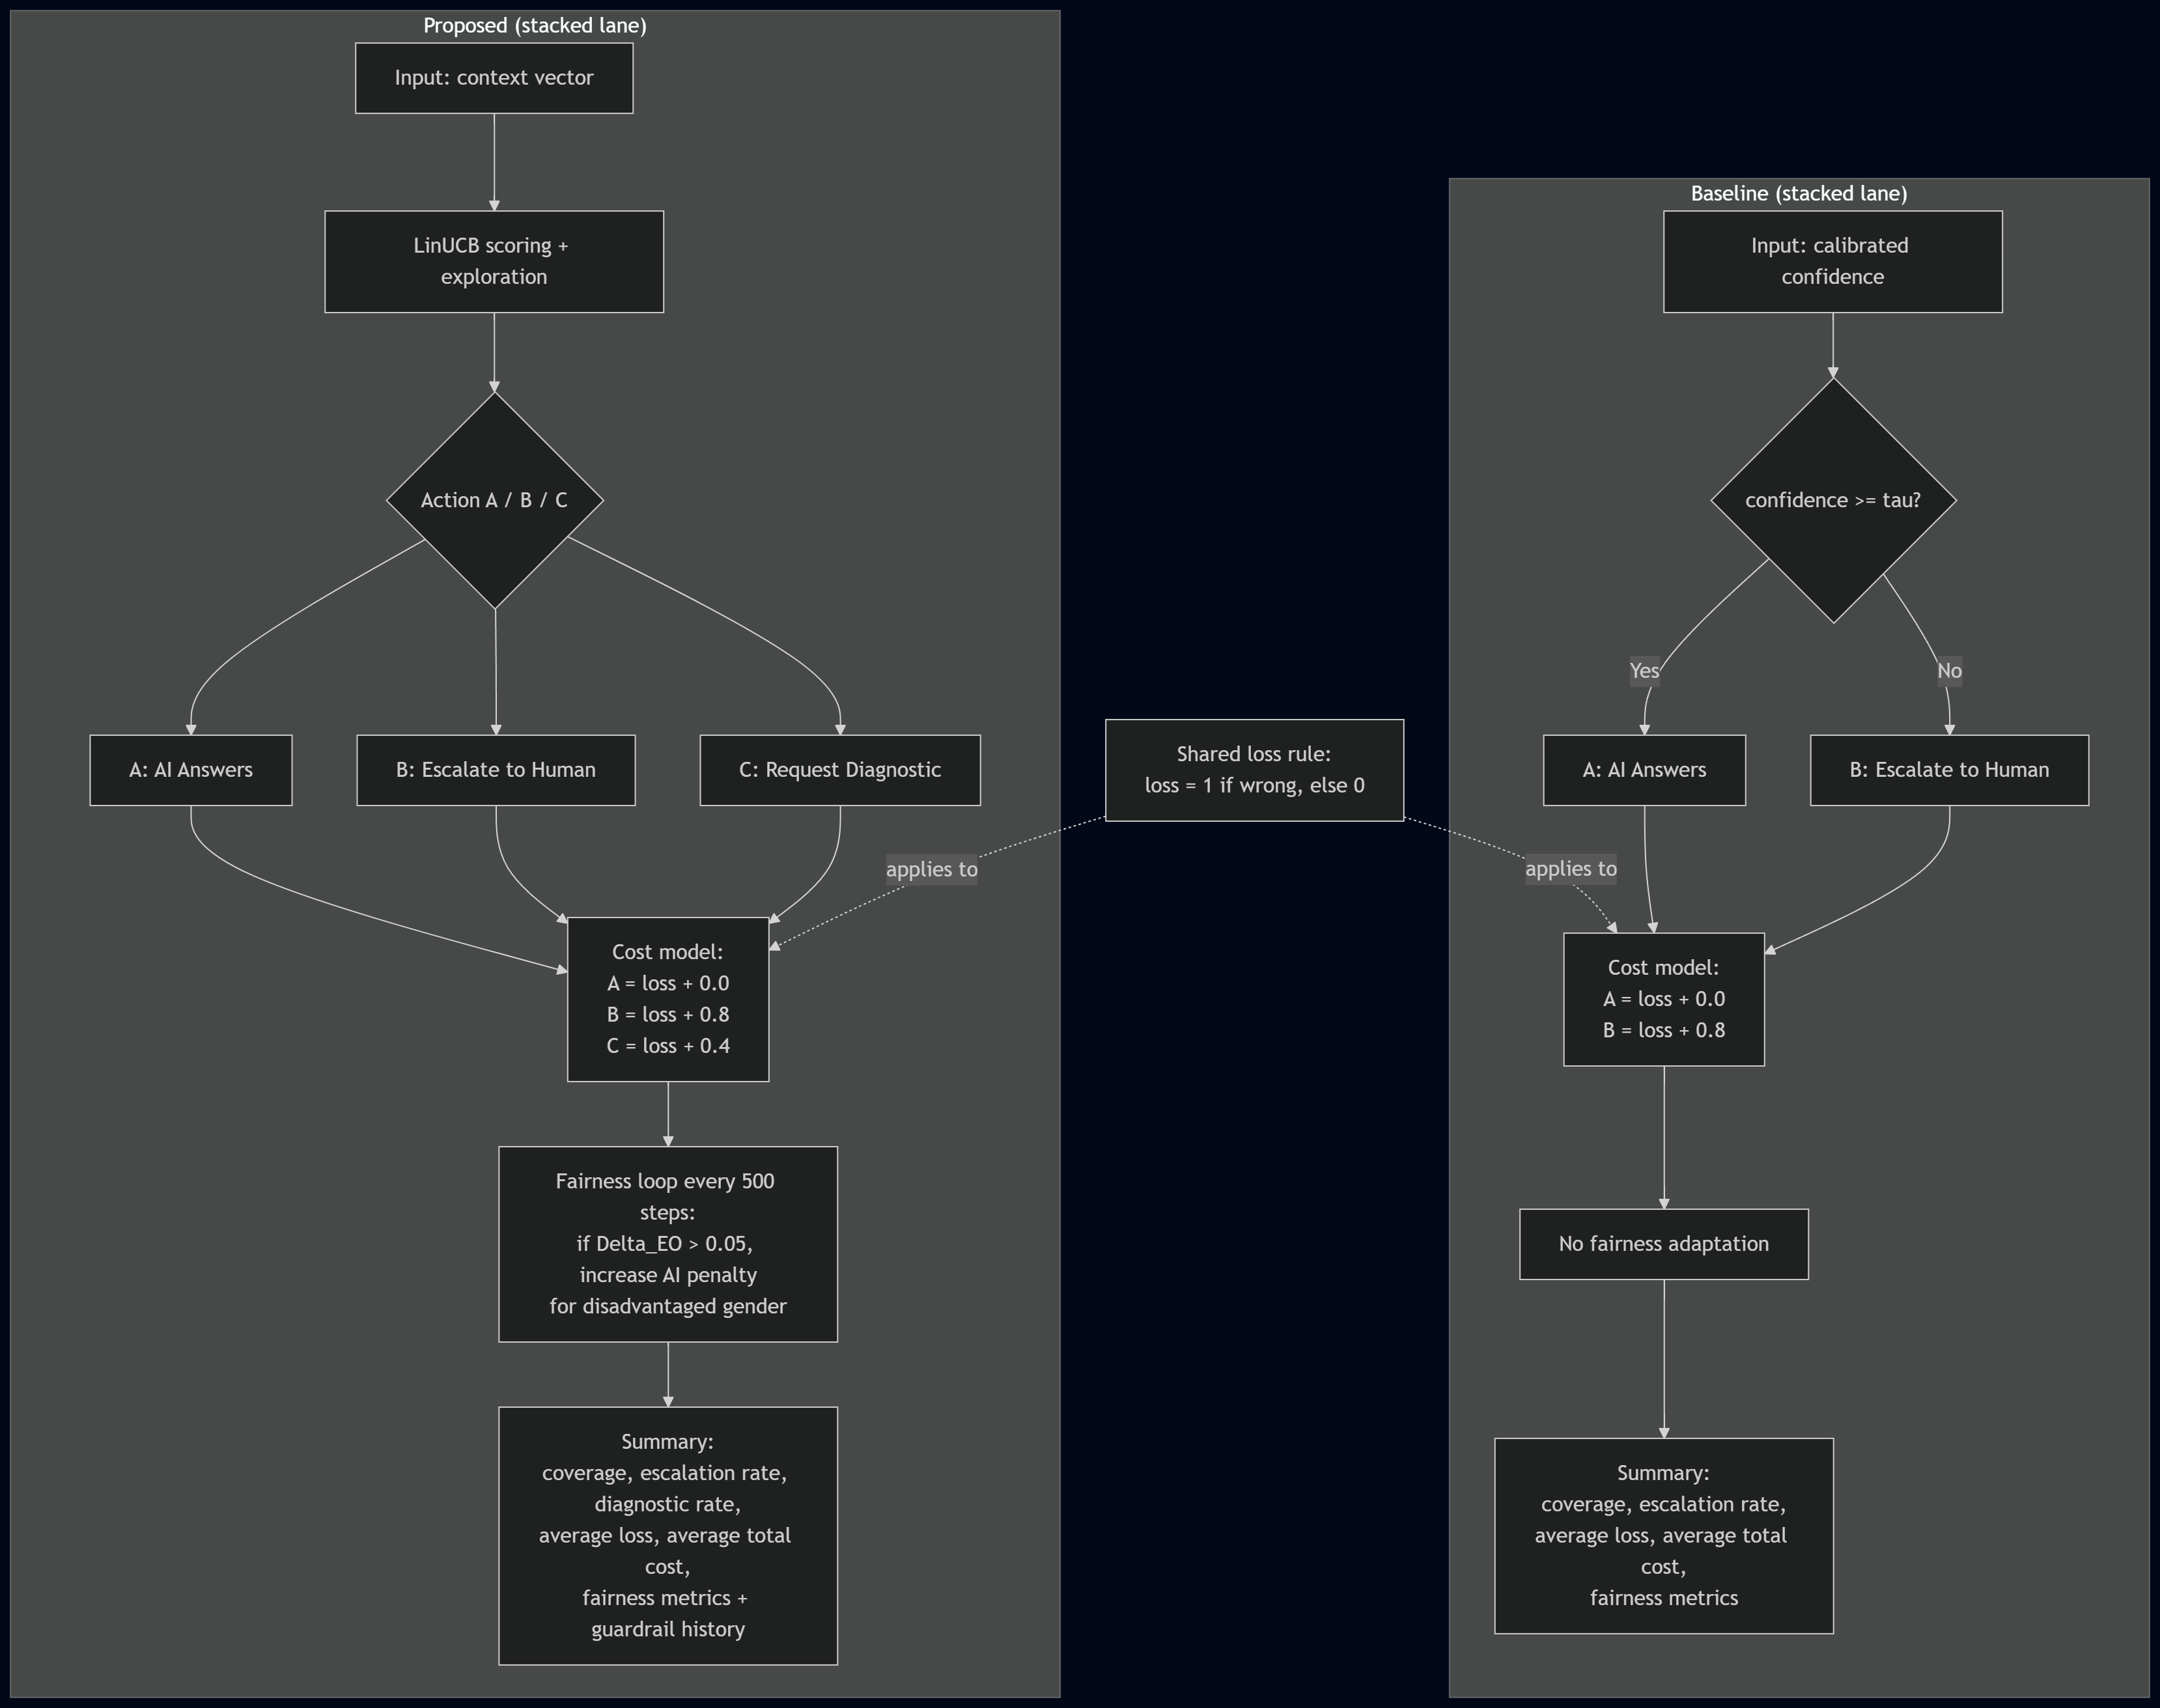
\includegraphics[width=0.98\linewidth]{../images/proposed_vs_baseline_flowchart.txt.png}}
    \caption{Baseline versus proposed workflow. The baseline routes only between AI and escalation by a confidence threshold, while the proposed policy uses contextual bandit routing with an additional diagnostic action and fairness guardrail updates.}
    \label{fig:policyflow}
\end{figure}

\section{Results}
Table~\ref{tab:main} shows the central deployment results. The adaptive policy substantially lowers deployment cost and closes the \emph{between-group} EO gap, but it also pushes escalation rates close to zero and increases task loss. This highlights the distinction between reducing disparity and providing sufficient absolute support coverage.

\begin{table}[t]
\centering
\caption{Main policy outcomes on a 180{,}000-step simulation stream (5x repeated test timeline).}
\label{tab:main}
\begin{tabular}{lcccccc}
\toprule
Policy & AI cov. & Escal. & Diag. & Avg loss & Avg total cost & $\Delta_{\text{EO}}$ \\
\midrule
Baseline & 0.798 & 0.202 & 0.000 & 0.202 & 0.384 & 0.0554 \\
Proposed & 0.9989 & 0.00009 & 0.0010 & 0.222 & 0.222 & 0.0035 \\
\bottomrule
\end{tabular}
\end{table}

Figure~\ref{fig:policyflow} summarizes the policy logic, Figure~\ref{fig:overall} reports overall risk--coverage behavior, and Figure~\ref{fig:transparency} shows the transparency artifacts used to audit decision rationale.

\begin{figure}[t]
    \centering
    
\includegraphics[width=0.95\linewidth]{../results_reframed_proficiency_5x/risk_coverage_overall.png}
    \caption{Overall risk--coverage curves. The adaptive policy operates at much higher AI coverage, reducing cost but with higher task loss.}
    \label{fig:overall}
\end{figure}

\begin{figure}[t]
    \centering
    
\includegraphics[width=0.49\linewidth]{../results_reframed_proficiency_5x/shap_global_importance.png}
    
\includegraphics[width=0.49\linewidth]{../results_reframed_proficiency_5x/shap_local_case.png}
    \caption{Transparency outputs: global SHAP importance (left) and local explanation for one escalated case (right).}
    \label{fig:transparency}
\end{figure}

\paragraph{Fairness.}
Compared with baseline, the proposed policy improves all tracked group fairness statistics:
EO gap (0.0554 \(\rightarrow\) 0.0035), equalized-odds difference (0.0554 \(\rightarrow\) 0.0035), and risk gap (0.0230 \(\rightarrow\) 0.00028) all improve. However, absolute FNR increases under the proposed policy (fewer false-negative disparities but more missed support overall), so parity improves more than absolute support quality.

\paragraph{Transparency.}
Global explanations indicate the strongest drivers are \texttt{attempt\_count}, rolling skill correctness, and recency, with skill-specific indicators contributing to finer adjustments. Local explanations for escalated cases expose why confidence was insufficient for autonomous action, supporting teacher oversight and accountability through SHAP-style additive attributions \citep{lundberg2017shap}.

\section{Discussion and limitations}
The key empirical insight is that deployment-aware routing can deliver large operational gains even when predictive risk worsens. In other words, optimizing end-to-end decision utility is not equivalent to optimizing classifier accuracy alone.

Limitations are important. First, human behavior is simulated; true classroom studies could produce different trade-offs. Second, gender is synthetic and used for methodological benchmarking, not sociological claims. Third, we evaluate one dataset and one model family; generalization to other subjects and cohorts remains open. Fourth, EO-gap control alone does not guarantee low harm for all students: in this run, subgroup parity improves but absolute false-negative rates remain high.

\section{Conclusion}
We implemented an end-to-end, reproducible human--AI collaboration pipeline for educational recommendation that integrates calibrated uncertainty, online routing, fairness monitoring, and transparency artifacts. Relative to a strong threshold baseline, the adaptive policy yields much lower deployment cost and stronger group fairness, while exposing a clear accuracy-cost-fairness trade-off that is central to responsible human--AI system design.

\section*{Reproducibility}
All artifacts (CSV logs, fairness tables, SHAP figures, and risk--coverage plots) are automatically generated by a single script (\texttt{run\_project.py}) and saved under \texttt{results\_reframed\_proficiency\_5x/} for this experiment. The run was executed on CPU in a Python virtual environment, using fixed random seed 42.

\bibliographystyle{plainnat}
\bibliography{references}

\appendix
\section{Additional implementation details}
The complete command used was:
\begin{verbatim}
/home/joelinator/env/bin/python run_project.py --simulation-timestep-multiplier 5 --results-dir results_reframed_proficiency_5x
\end{verbatim}
The script downloads ASSISTments data if absent, preprocesses it into
\texttt{data/assistments\_2009\_processed\_with\_gender.csv}, and then produces all metrics and figures.

\newpage
\input{checklist.tex}

\end{document}
